\documentclass[12pt]{article}

% load packages 
\usepackage{mathptmx}
\usepackage{geometry}
\usepackage{graphicx}
\usepackage{wrapfig}
\usepackage{afterpage}
\usepackage{natbib}
\usepackage{setspace}
\usepackage{abstract}
\usepackage{tocloft}
\usepackage[toc, page, title]{appendix}
\usepackage{multirow}
\usepackage{tabularx}
\usepackage{float}
\usepackage{subcaption}
\usepackage{indentfirst}
\usepackage{sectsty}

% page layout
\geometry{margin=0.8in}
\renewcommand{\arraystretch}{1.5} 
\setlength\parindent{20pt}\setlength{\parskip}{0.0pt plus 0.0pt}

% text formatting
\sectionfont{\large \scshape}
\subsectionfont{\normalsize\itshape}
\subsubsectionfont{\normalsize\mdseries\itshape}
\setcounter{secnumdepth}{3}
\renewcommand{\abstractname}{Résumé}
\setlength{\abstitleskip}{-0.5em}
\renewcommand{\abstractnamefont}{\normalfont \large \bfseries \scshape}
\renewcommand{\abstracttextfont}{\normalfont \normalsize}
\renewcommand\refname{Bibliographie}
\renewcommand{\contentsname}{Sommaire}
\renewcommand{\listfigurename}{Liste des Figures}
\renewcommand{\listtablename}{Liste des Tableaux}
\renewcommand{\appendixtocname}{Annexes}
\renewcommand{\appendixpagename}{\large \scshape \bfseries Annexes}
\renewcommand{\appendixname}{Annexe}
\renewcommand{\setthesection}{\Alph{section}}


% toc formatting
\setlength\cftsecindent{0pt}
\setlength\cftsubsecindent{20pt}
\setlength\cftsubsubsecindent{48pt}
\setlength\cftbeforesecskip{18pt}
\setlength\cftbeforesubsecskip{10pt}
\setlength\cftbeforesubsubsecskip{8pt}
\renewcommand{\cftdot}{.}
\renewcommand{\cfttoctitlefont}{\large \scshape \bfseries}
\renewcommand{\cftloftitlefont}{\large \scshape \bfseries}
\renewcommand{\cftlottitlefont}{\large \scshape \bfseries}
\renewcommand{\cftpnumalign}{l}
\setlength{\cftbeforefigskip}{5pt}
\cftsetpnumwidth{50pt}
\cftsetrmarg{65pt}

% biblio style
\setcitestyle{authoryear,open={(},close={)}}

% figure and table
\floatplacement{figure}{h}
\floatplacement{table}{h}
\setlength\columnsep{20pt}

% empty page
\newcommand\myemptypage{
    \null
    \thispagestyle{empty}
    \addtocounter{page}{-1}
    \newpage
    }


\begin{document}
\begin{titlepage}
\centering
\includegraphics[width=8cm]{img/amu-logo.png}\hfill  \includegraphics[width=4.2cm]{img/logo-ofb.png} \hfill \includegraphics[width=3.7cm]{img/logo-mio.png}\par\vspace{1cm}
{\scshape\large Aix-Marseille Université\par}
{\large Institut OSU-Pythéas\par}
Institut Méditerranéen d’Océanologie - MIO \par
\vspace{2cm}
{\scshape\large Master Sciences de la mer\par}
{\large Parcours Océanographie Biologique et Écologie Marine\par}
\vspace{2cm}
{\LARGE \bfseries Titre du stage\par}
\vspace{.5cm}
{\large \itshape Couteyen Carpaye, Mathilde\par}
\vfill
{\itshape Etude réalisée au sein de l'Institut Méditerranéen d'Océanologie\par}
{\itshape Sous la direction de M. Gérald Grégori et M. David Nérini\par }
\vfill
Année universitaire\par
2021-2022
\end{titlepage}

\myemptypage

\section*{Remerciements}


\newpage


\newpage
\tableofcontents
\newpage


\section{Introduction}


\section{Matériels \& Méthodes}

\subsection{SOMLIT (Service d'Observation en Milieu LITtoral)}

\subsubsection{Les stations}

\subsubsection{Prélèvements et protocoles}

\subsubsection{Jeux de données}

\begin{figure}
\centering
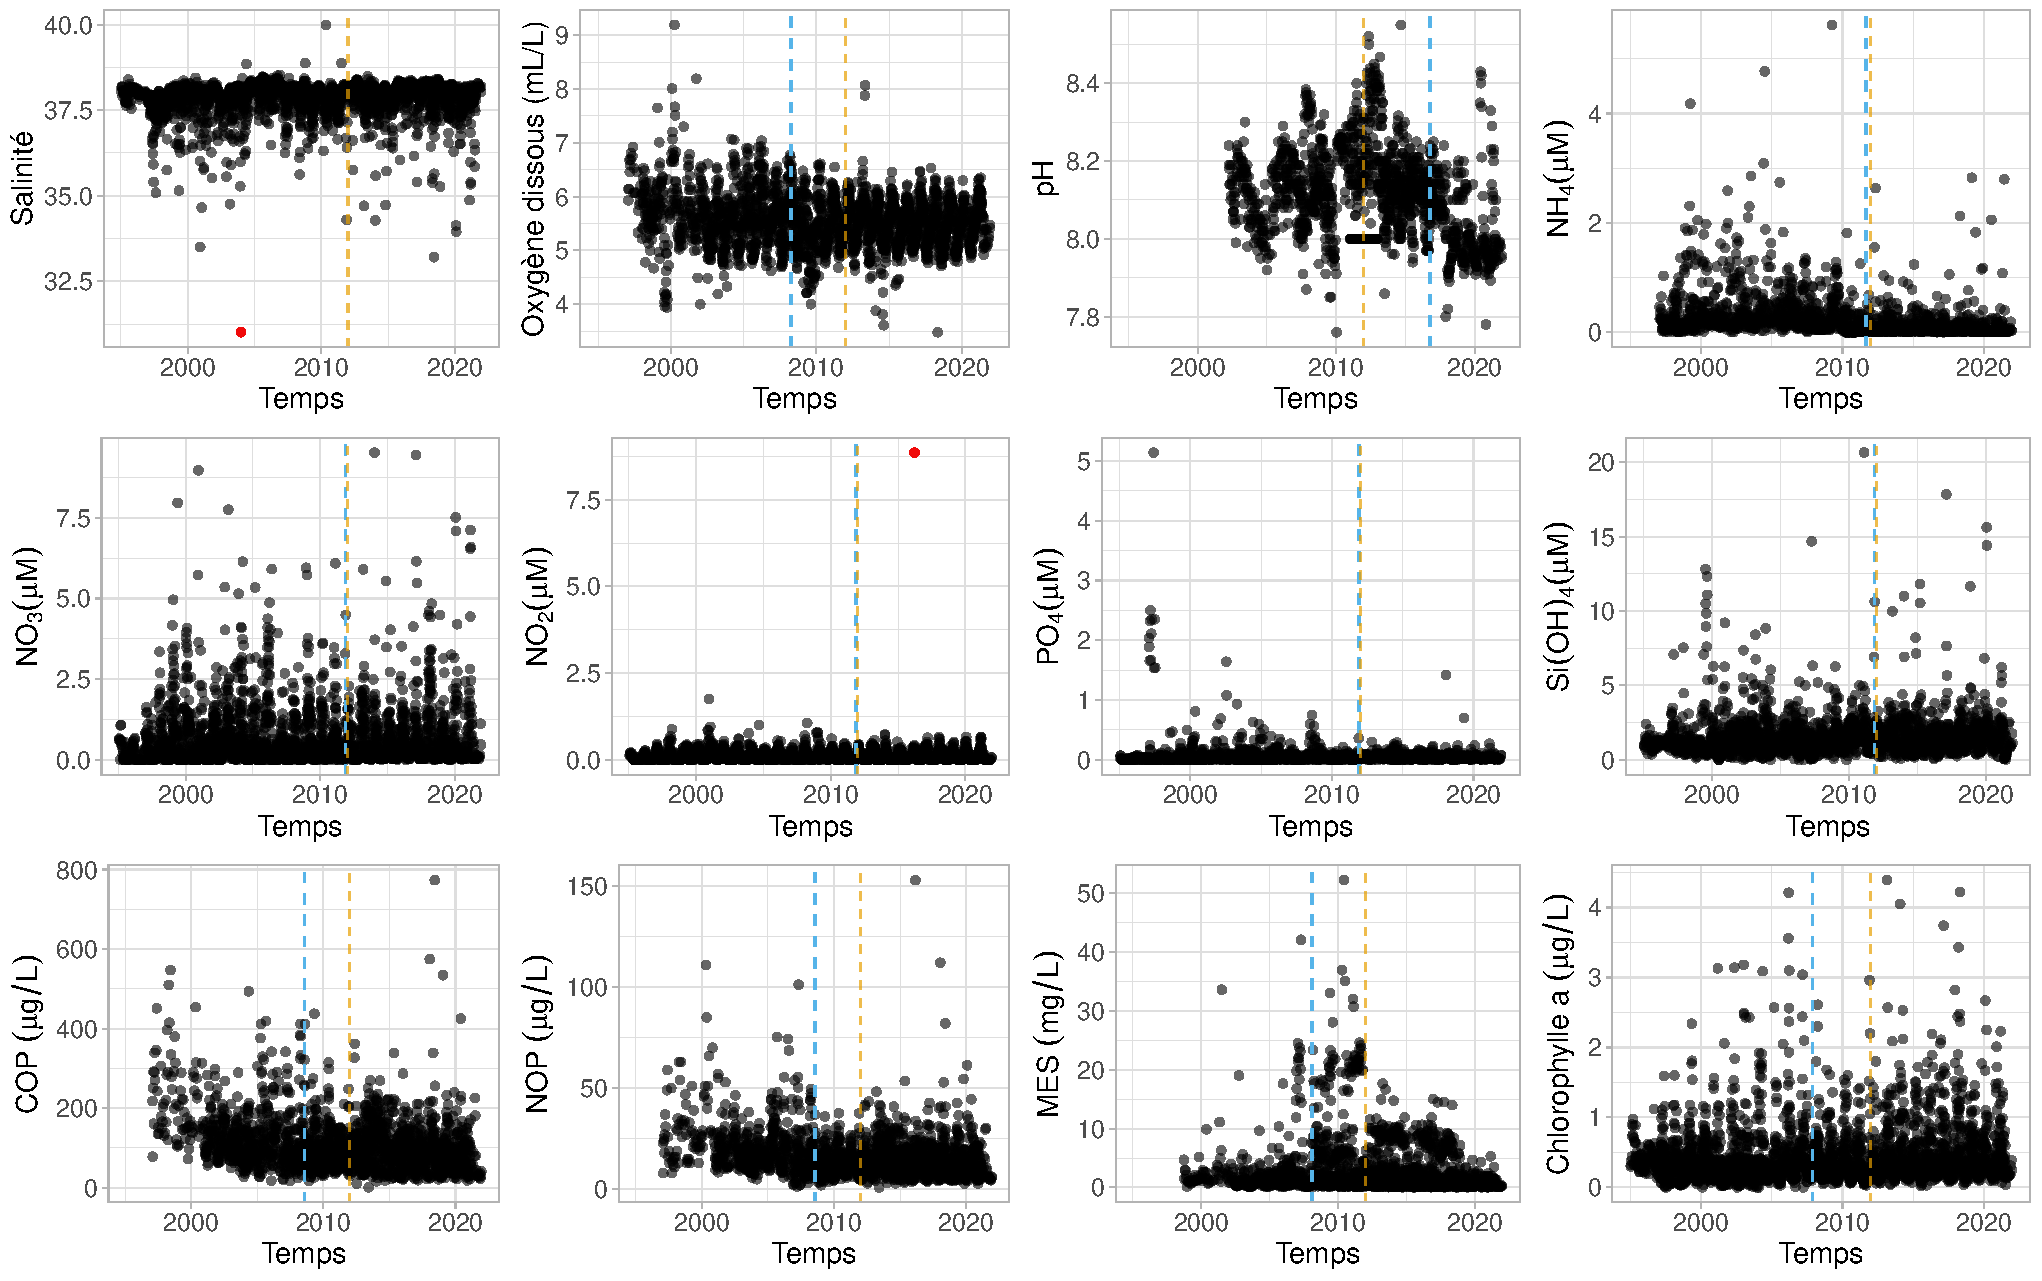
\includegraphics[width=\textwidth]{fig/visualisation_hydro.pdf}
\caption{Séries temporelles des données hydrologiques de surface pour les trois stations SOMLIT méditerranéennes confondues. La ligne pointillé bleue correspond à la mise en place du protocole national pour la variable présentée. La ligne pointillée orange correspond au début du jeu de données PICONANO. Les éventuelles données aberrantes sont représentées en rouge.}
\end{figure}

\begin{figure}
\centering
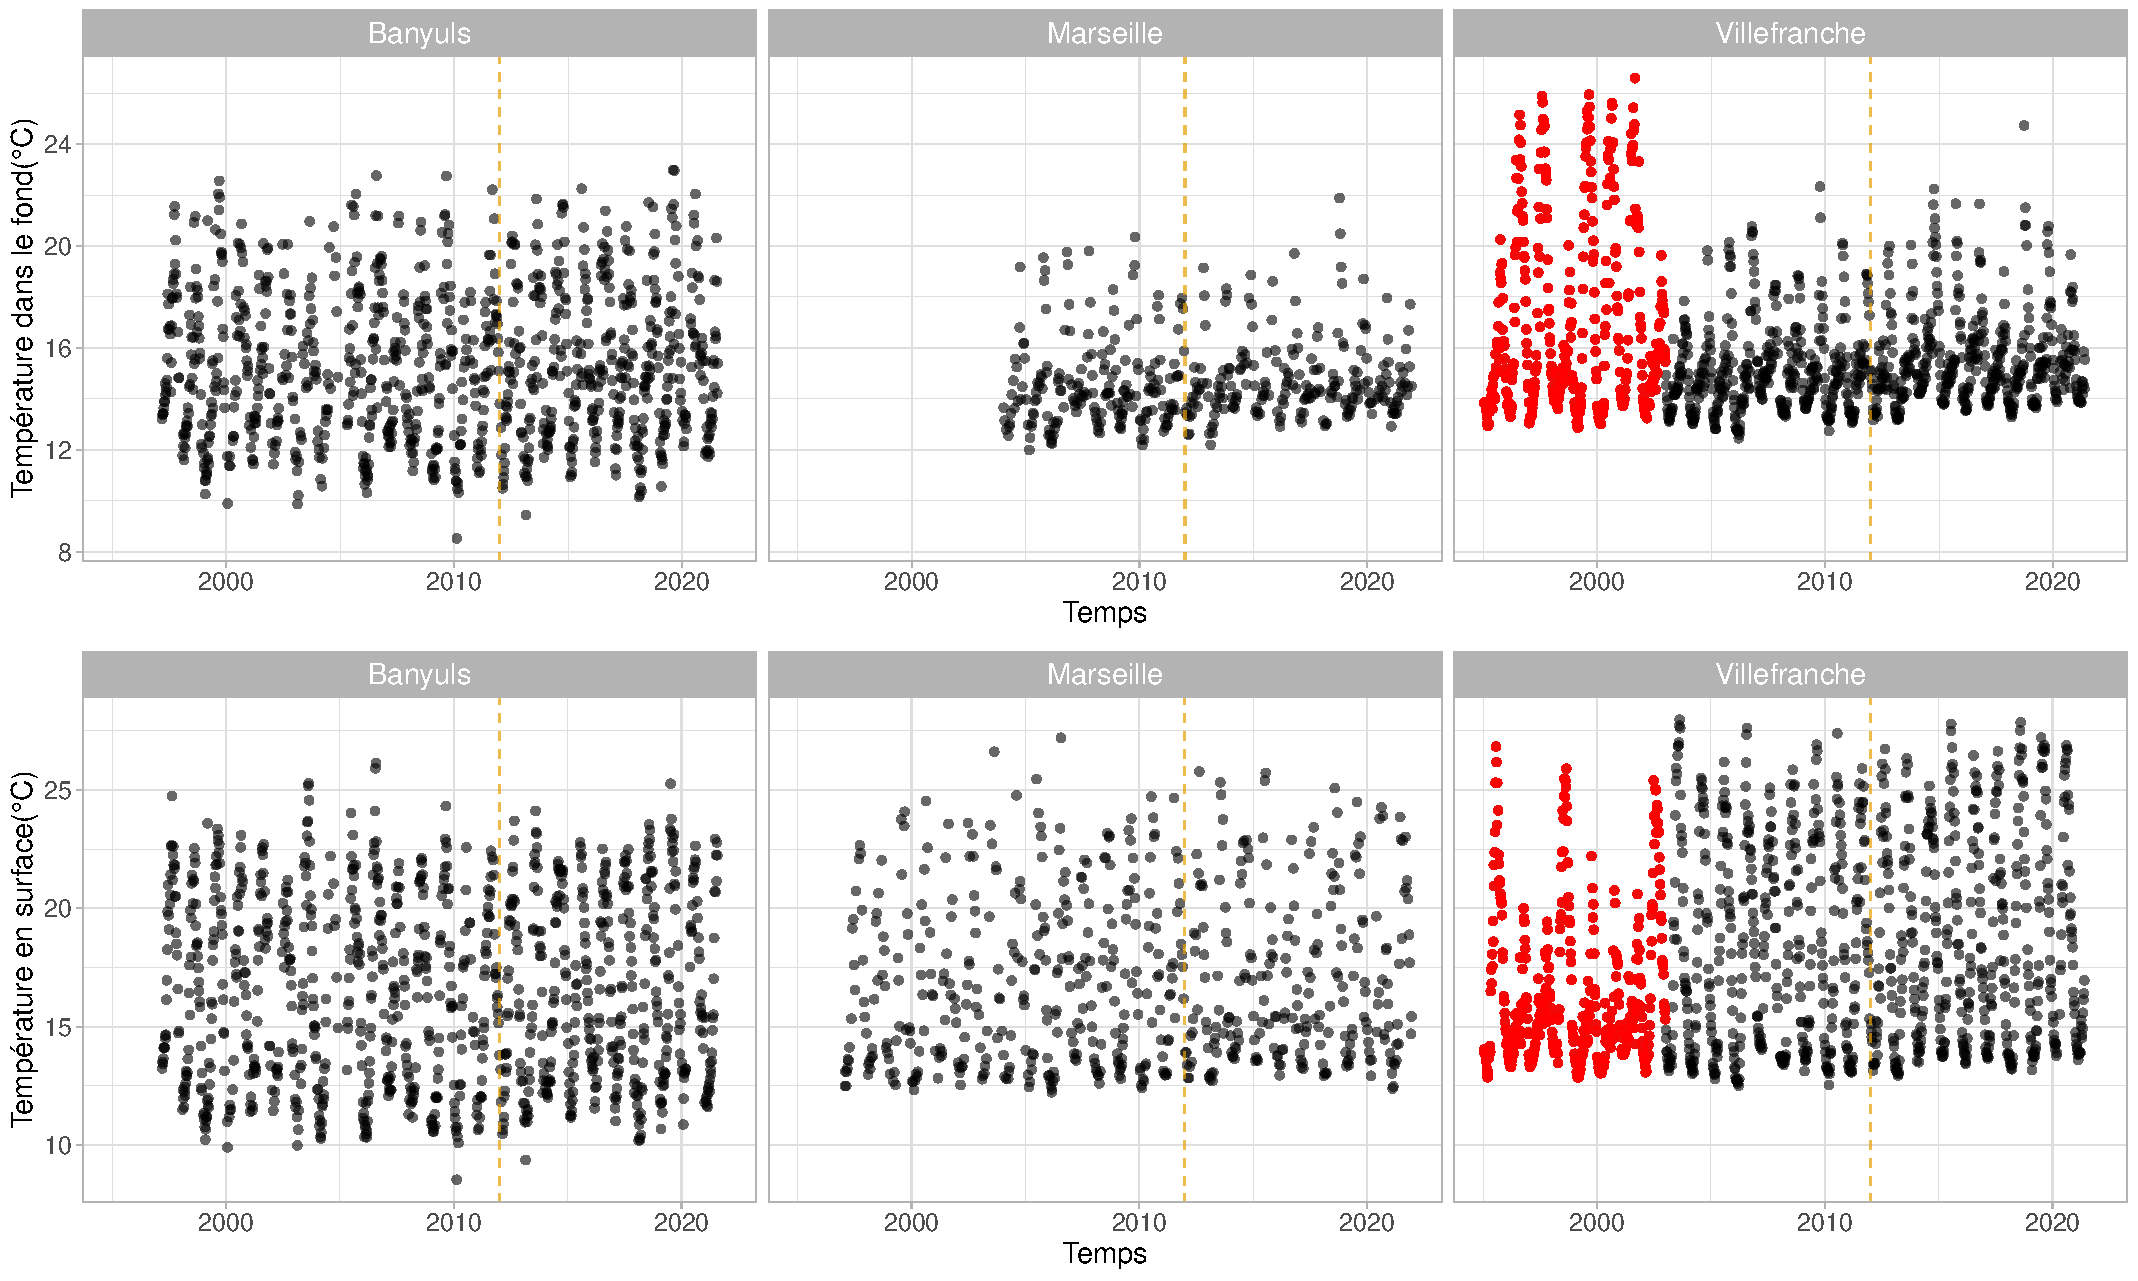
\includegraphics[width=.9\textwidth]{fig/visualisation_T.pdf}
\caption{Séries temporelles des données de Température en surface et au fond pour les trois stations méditerranéennes. La ligne pointillée orange correspond au début du jeu de données PICONANO. Les éventuelles données aberrantes sont représentées en rouge.}
\end{figure}


\begin{figure}
\centering
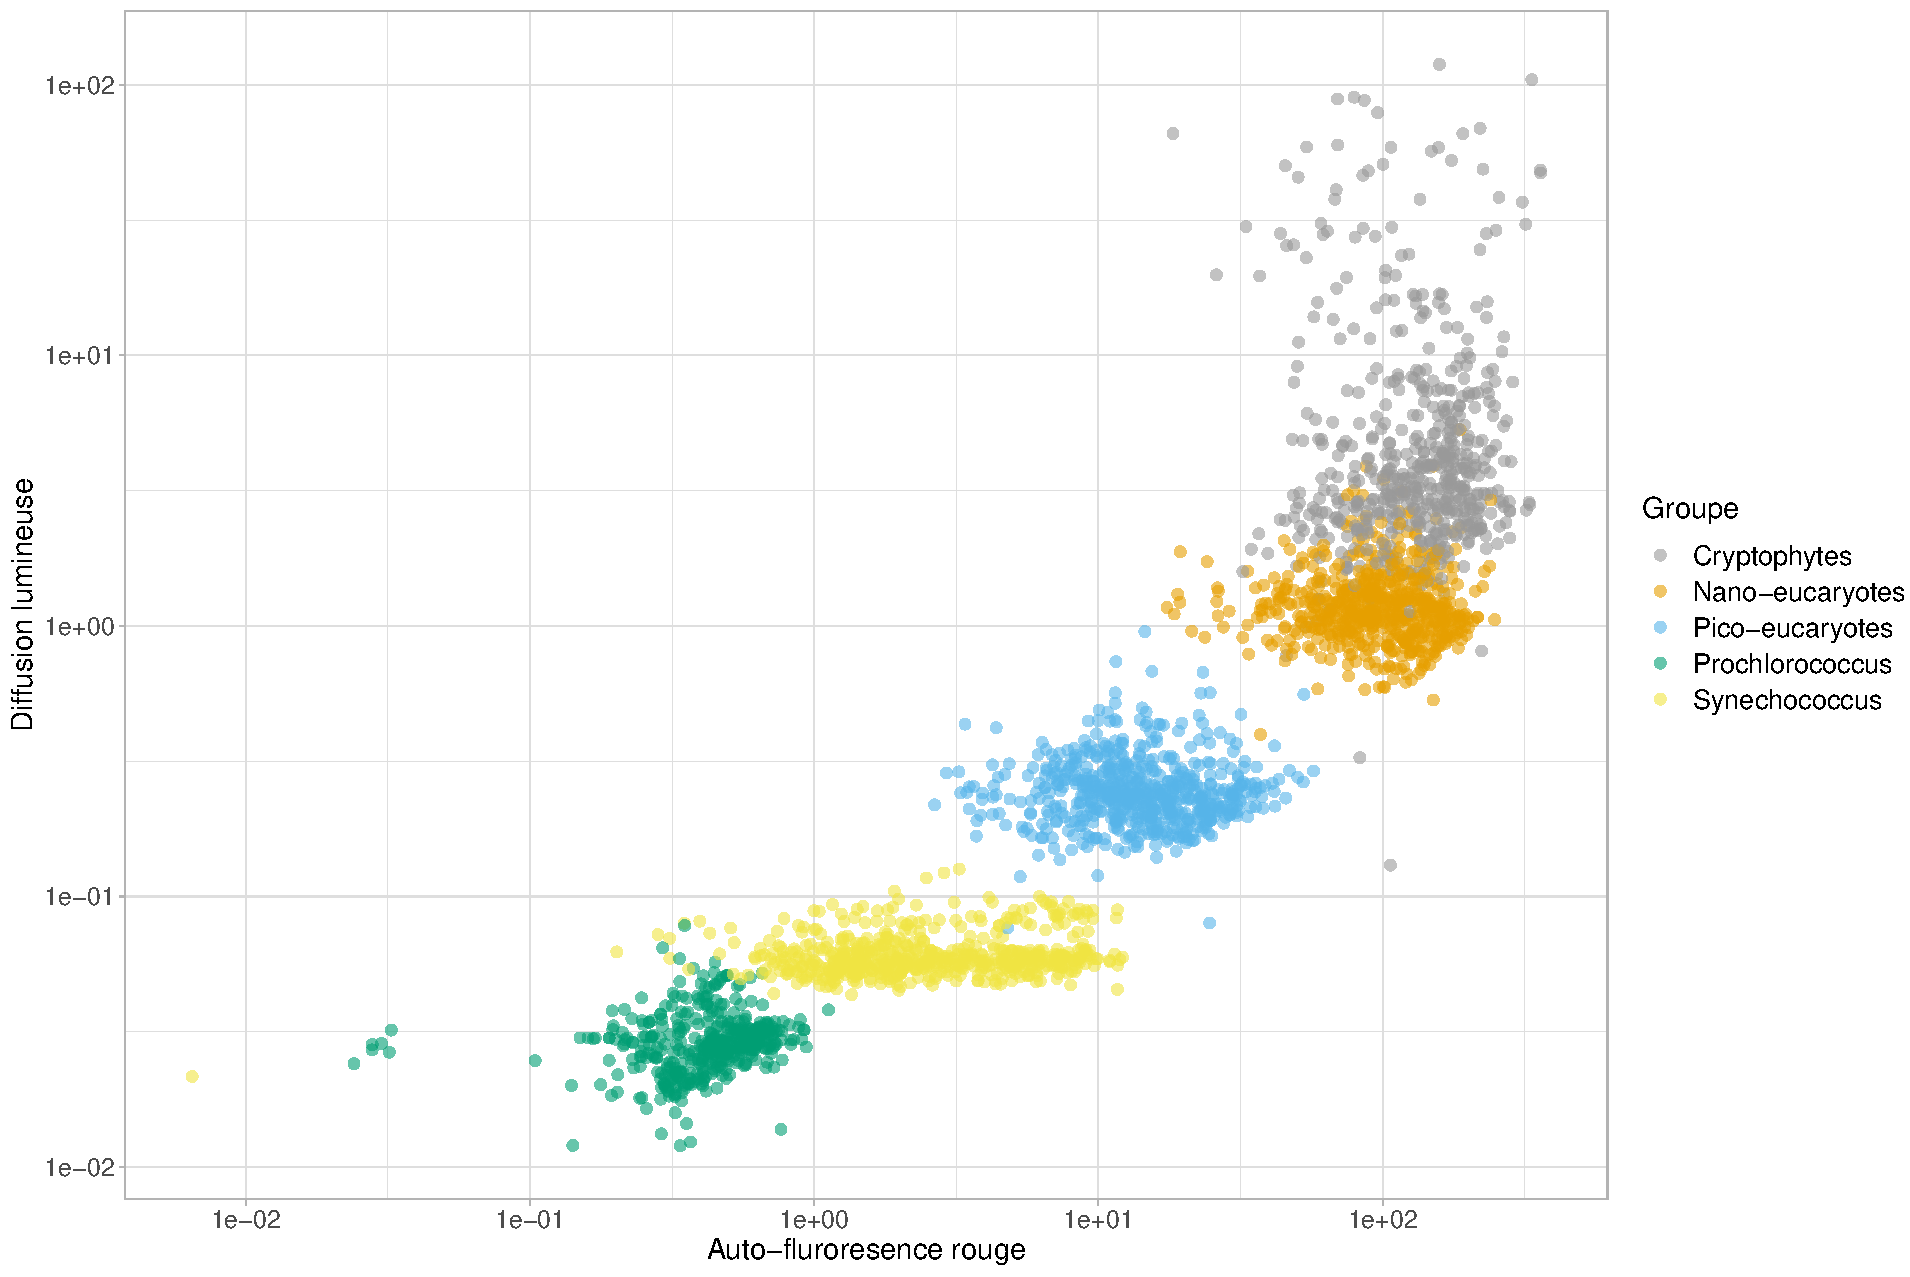
\includegraphics[width=.75 \textwidth]{fig/visualisation_phyto.pdf}
\caption{}
\end{figure}

\begin{figure}
\centering
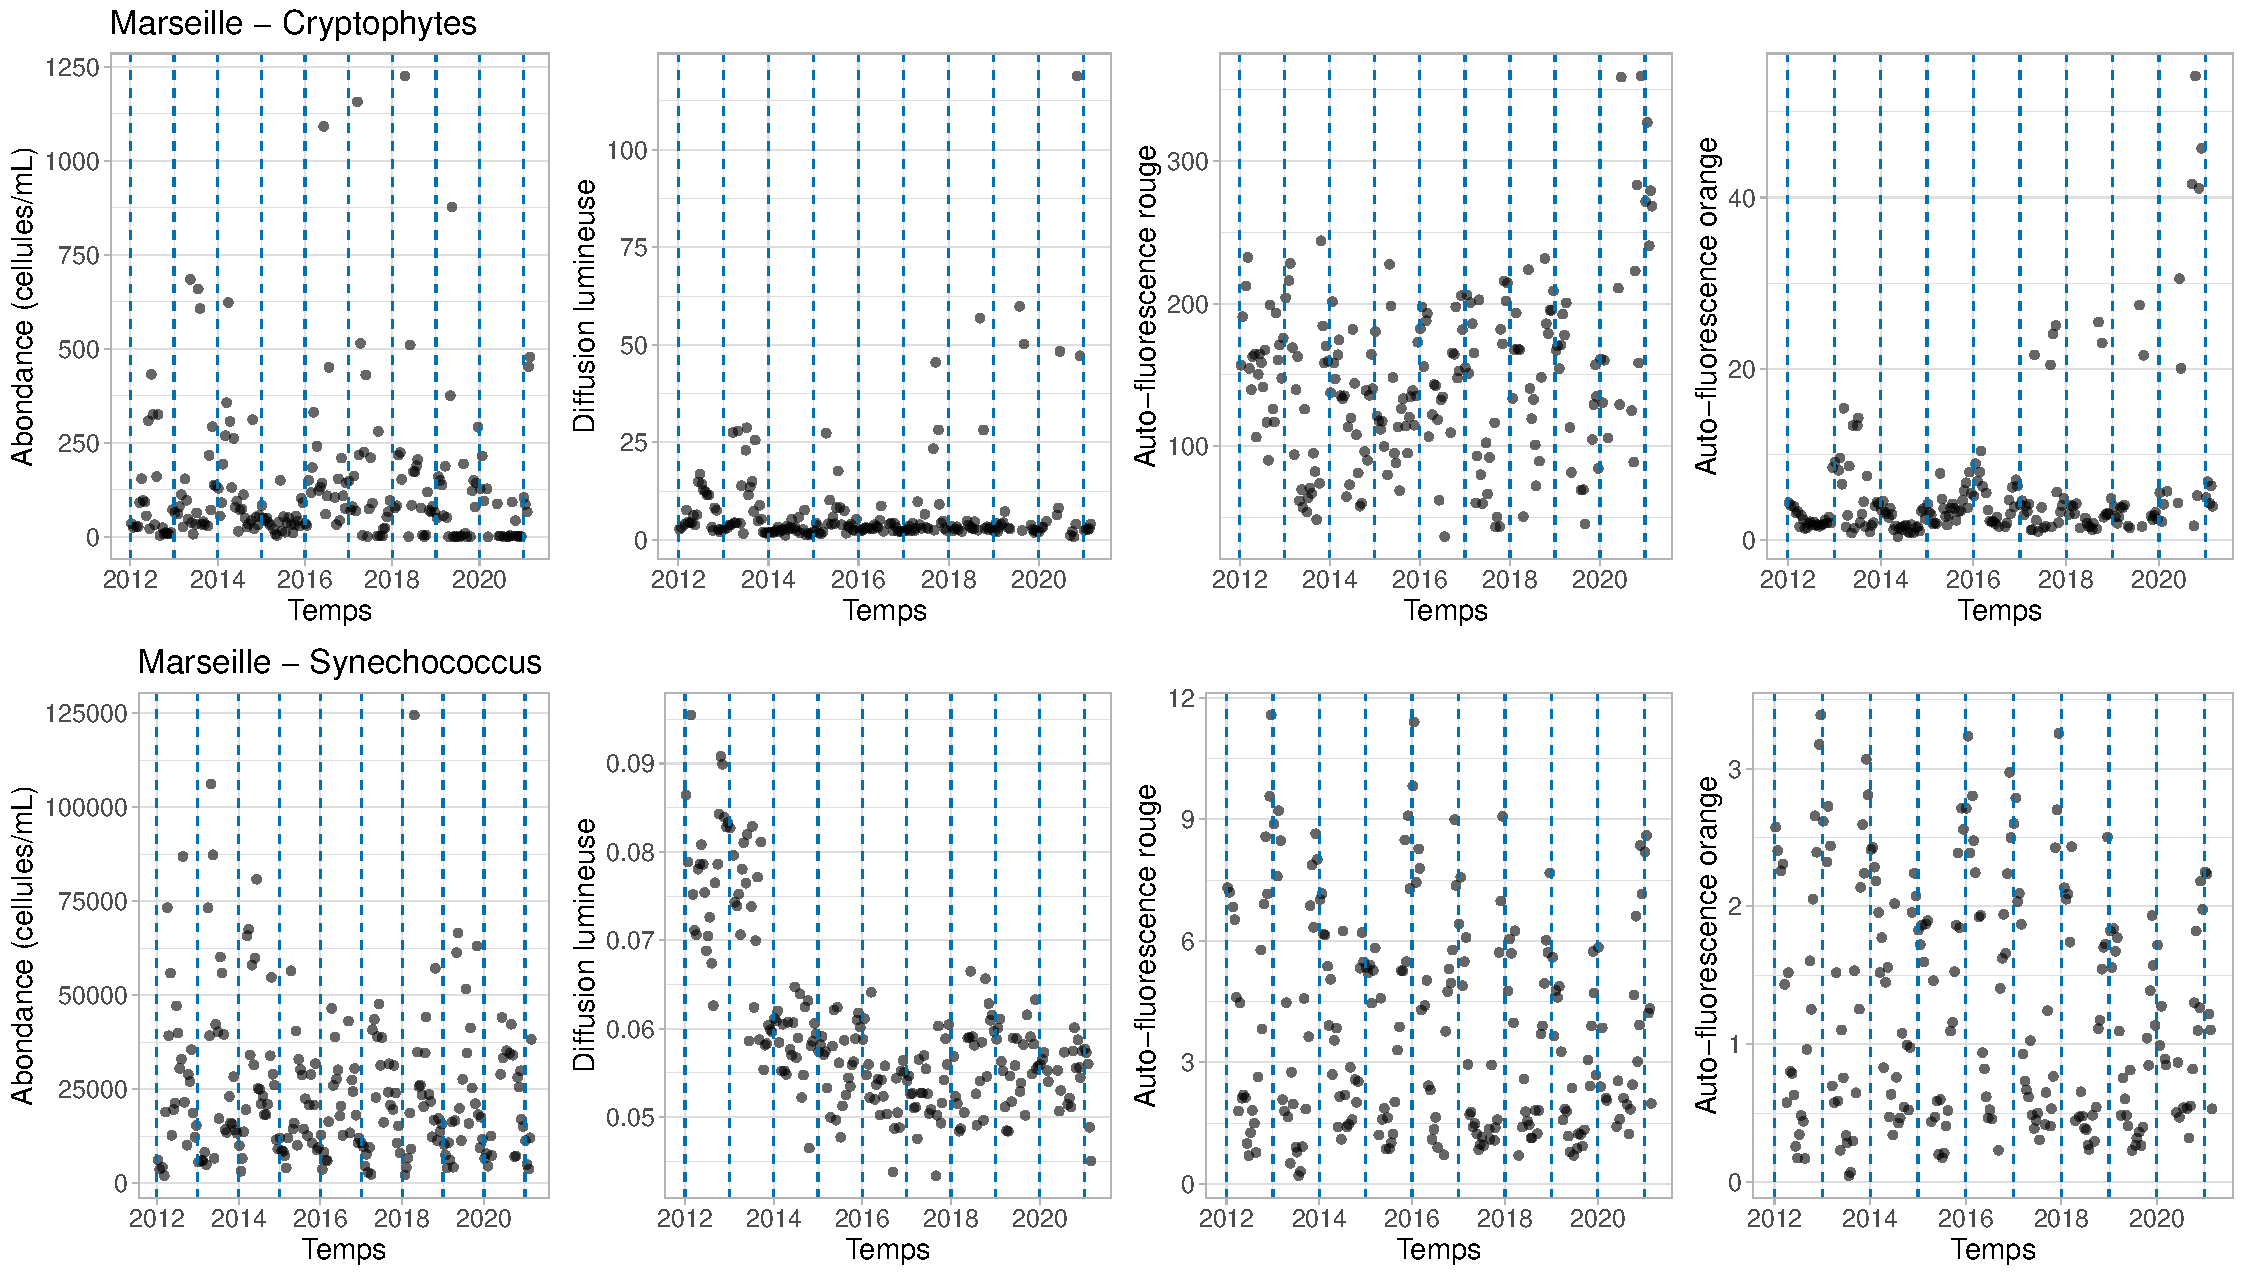
\includegraphics[width=\textwidth]{fig/visualisation_cyano.pdf}
\caption{Série temporelle des données de cytométrie pour Prochlorococcus et Synechococcus pour la station de Marseille. Les lignes pointillées bleues correspondent au 1er janvier de chaque année.}
\end{figure}




\section{Résultats}



\section{Discussion}



\section{Conclusion}


\addcontentsline{toc}{section}{Bibliographie}
\bibliography{biblio}

\newpage
\addcontentsline{toc}{section}{Liste des Figures}
\listoffigures

\addcontentsline{toc}{section}{Liste des Tableaux}
\listoftables

\newpage
\begin{appendices}

\end{appendices}


\begin{abstract}

\end{abstract}

\end{document}
